\documentclass[pdflatex,compress,mathserif]{beamer}

%\usetheme[dark,framenumber,totalframenumber]{ElektroITK}
\usetheme[darktitle,framenumber,totalframenumber]{ElektroITK}

\usepackage[utf8]{inputenc}
\usepackage[T1]{fontenc}
\usepackage{lmodern}
\usepackage[english]{babel}
\usepackage{amsmath}
\usepackage{amsfonts}
\usepackage{amssymb}
\usepackage{graphicx}
\usepackage{multicol}
\usepackage{lipsum}
\usefonttheme[onlymath]{serif}

\newcommand*{\Scale}[2][4]{\scalebox{#1}{$#2$}}%

\setbeamertemplate{caption}[numbered]

\title{Digital Signal Processing}

\subtitle{Introduction}

\date{August, $7^{th}$ 2023}

\author{Mifta Nur Farid}

\begin{document}

\maketitle

\section{Basic concepts of digital signal processing}

\begin{frame}{A digital signal processing scheme}
	\begin{figure}
		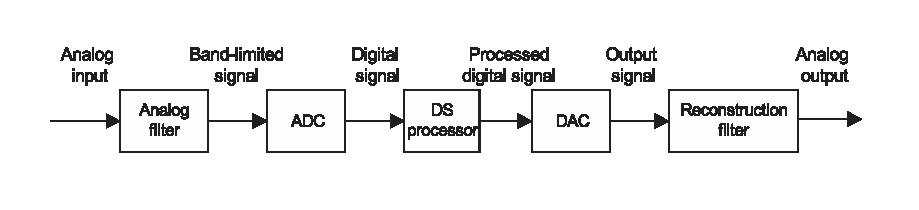
\includegraphics[width=\linewidth]{img/img01}
	\end{figure}
\end{frame}

\section{Basic digital signal processing examples in block diagrams}

\subsection{Digital filtering}

\begin{frame}{The simple digital filtering block}
	\begin{figure}
		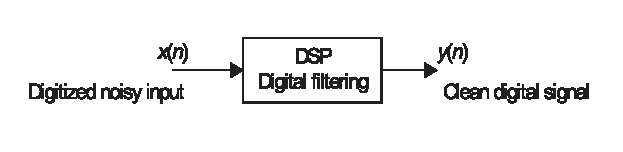
\includegraphics[width=\linewidth]{img/img02}
	\end{figure}
\end{frame}

\begin{frame}{Digitized noisy signal and clean digital signal using the digital lowpass filter}
	\begin{figure}
		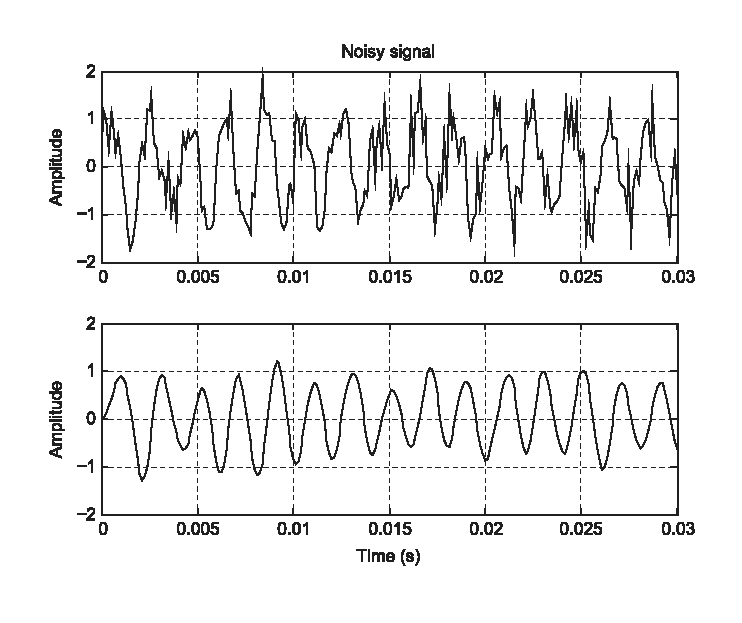
\includegraphics[width=0.8\linewidth]{img/img03}
	\end{figure}
\end{frame}

\subsection{Signal frequency (spectrum) analysis}

\begin{frame}{Signal spectral analysis}
	\begin{figure}
		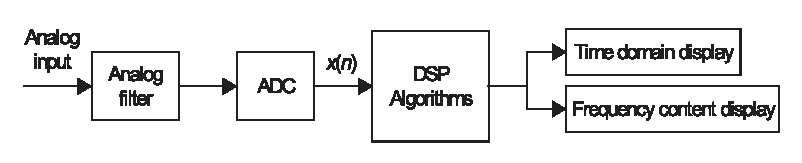
\includegraphics[width=\linewidth]{img/img04}
	\end{figure}
\end{frame}

\begin{frame}{Audio signals and their spectra}
	\begin{figure}
		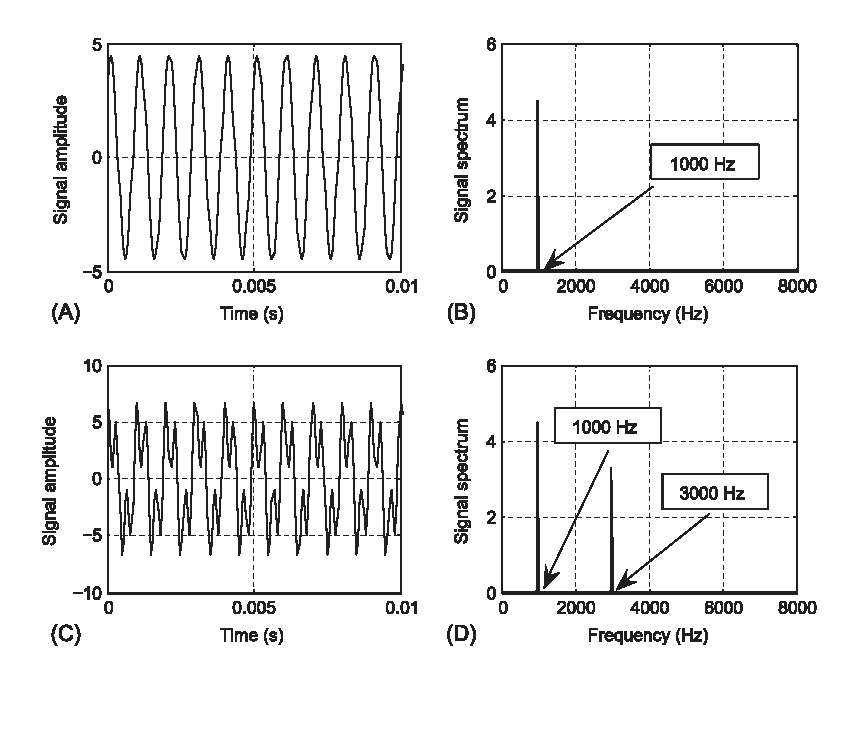
\includegraphics[width=0.8\linewidth]{img/img05}
	\end{figure}
\end{frame}

\begin{frame}{Speech samples and speech spectrum}
	\begin{figure}
		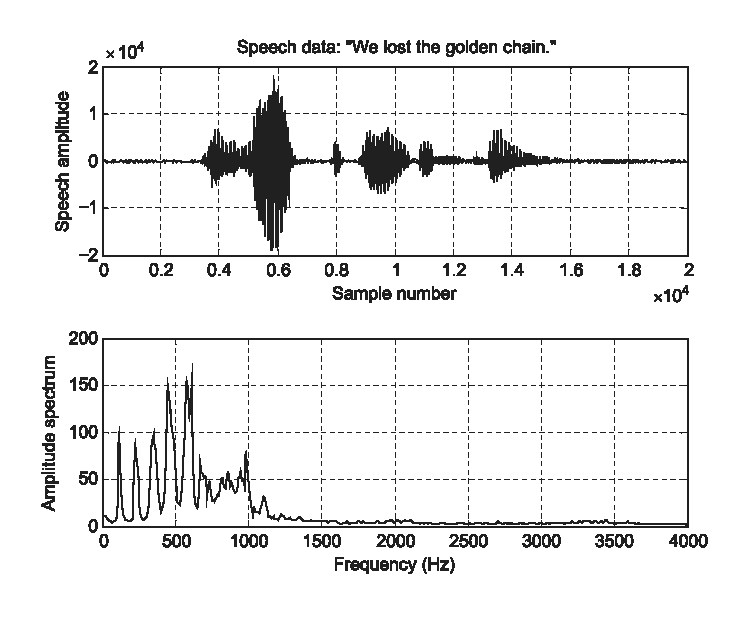
\includegraphics[width=0.8\linewidth]{img/img06}
	\end{figure}
\end{frame}

\section{Overview of typical digital signal processing in real-world applications}

\subsection{Digital crossover audio system}

\begin{frame}{Two-band digital crossover}
	\begin{figure}
		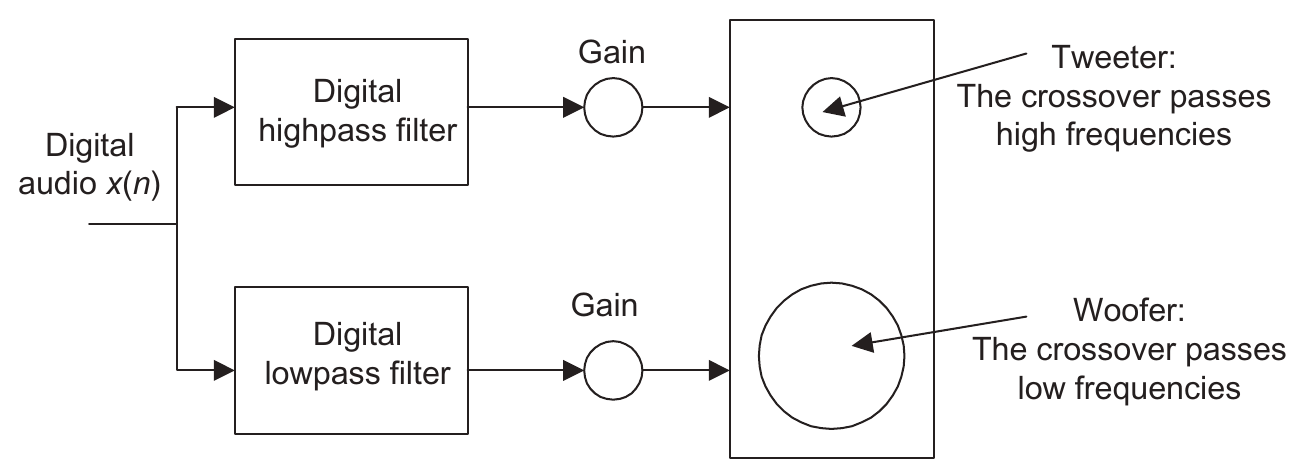
\includegraphics[width=0.8\linewidth]{img/img07}
	\end{figure}
\end{frame}

\subsection{Interference cancellation in electrocardiography}

\begin{frame}{Elimination of 60-Hz interference in electrocardiography (ECG)}
	\begin{figure}
		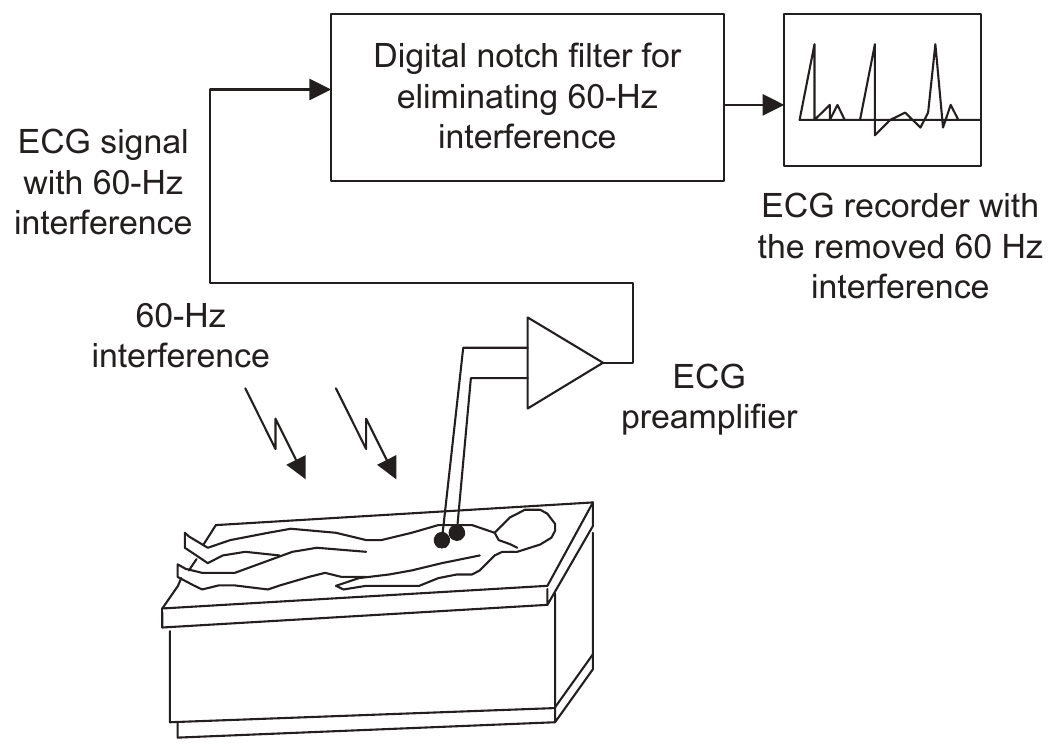
\includegraphics[width=0.8\linewidth]{img/img08}
	\end{figure}
\end{frame}

\subsection{Speech coding and compression}

\begin{frame}{Simplified data compressor and data expander (decompressor)}
	\begin{figure}
		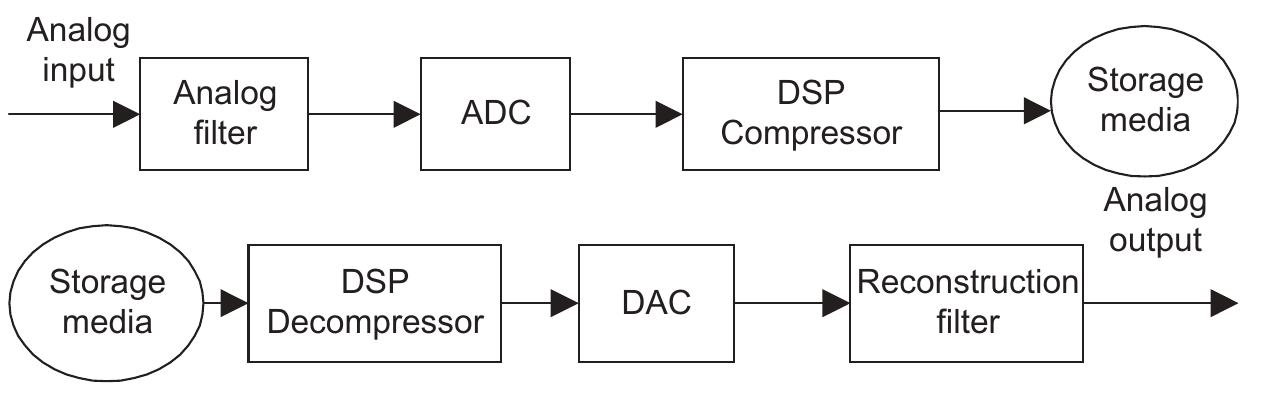
\includegraphics[width=0.8\linewidth]{img/img09}
	\end{figure}
\end{frame}

\subsection{Compact-disc recording system}

\begin{frame}{Simplified encoder of the CD\\recording system and decoder of\\the CD recording system}
	\begin{figure}
		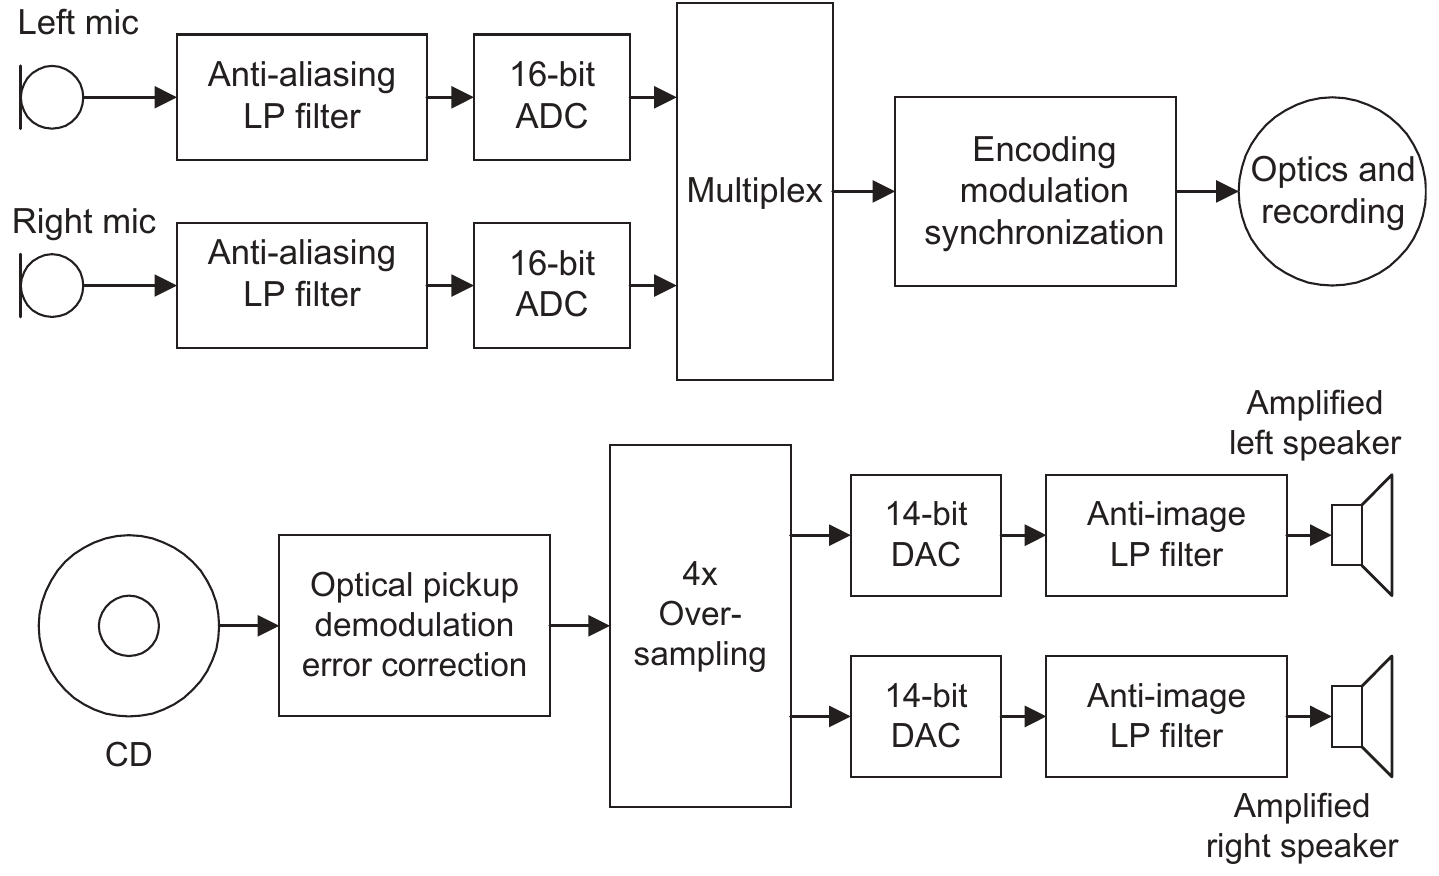
\includegraphics[width=0.7\linewidth]{img/img10}
	\end{figure}
\end{frame}

\subsection{Vibration signature analysis for defected gear tooth}

\begin{frame}{Vibration signature analysis of the gearbox}
	\begin{figure}
		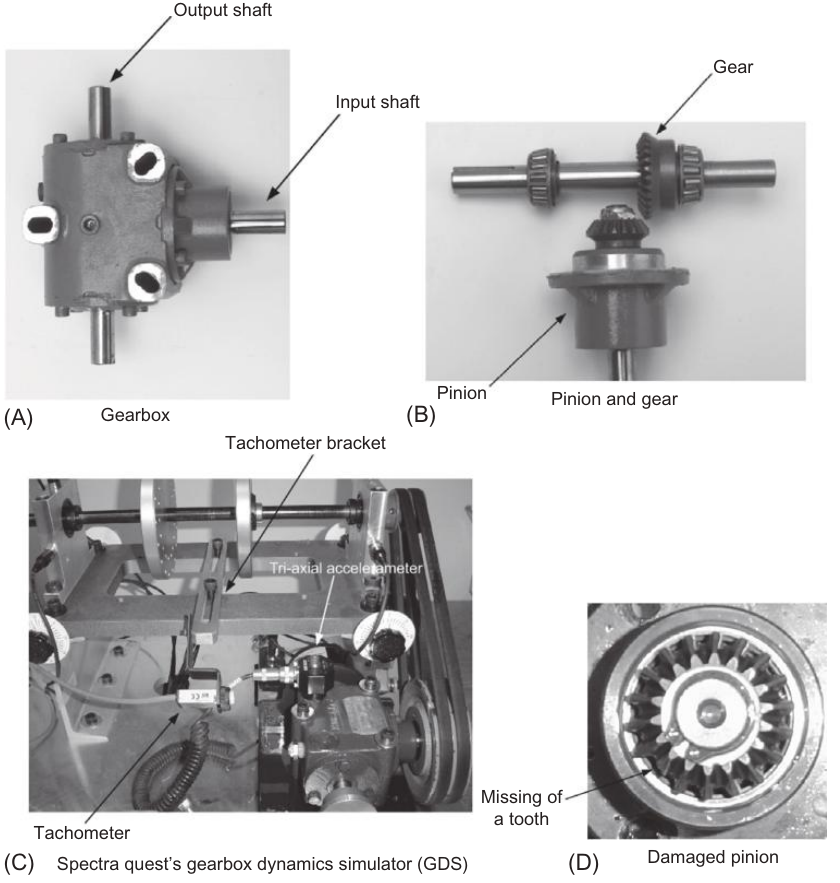
\includegraphics[width=0.5\linewidth]{img/img11}
	\end{figure}
\end{frame}

\begin{frame}{Vibration signal and spectrum\\from the good condition gearbox}
	\begin{figure}
		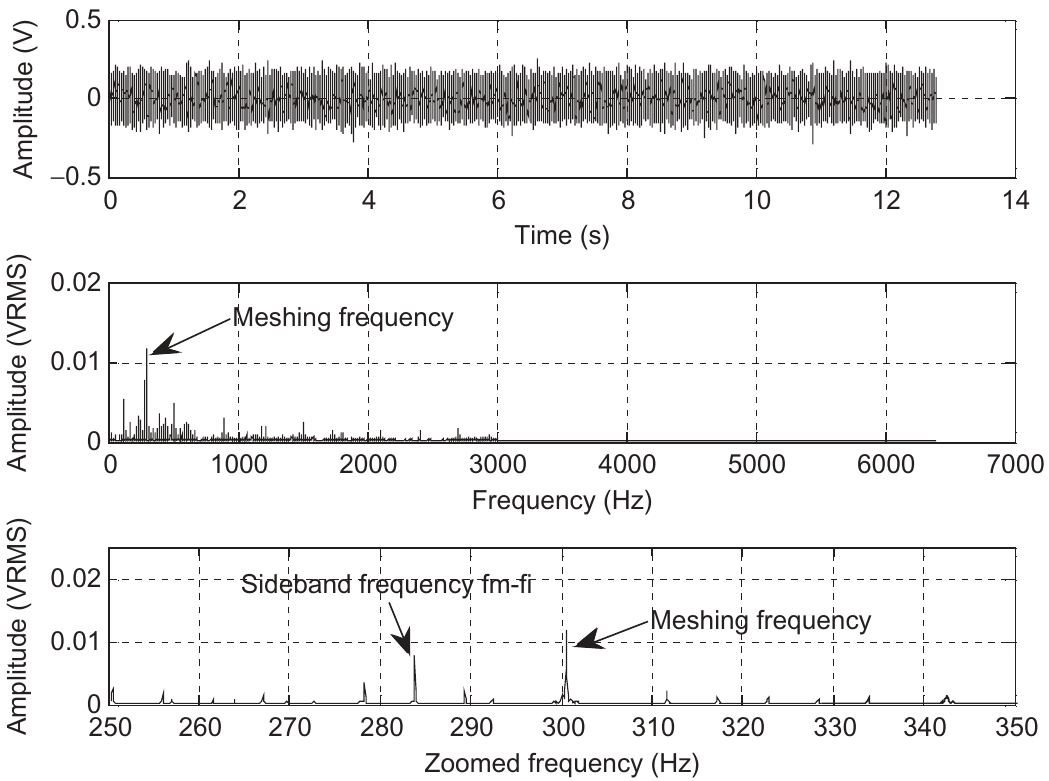
\includegraphics[width=0.8\linewidth]{img/img12}
	\end{figure}
\end{frame}

\begin{frame}{Vibration signal and spectrum\\from the damaged gearbox}
	\begin{figure}
		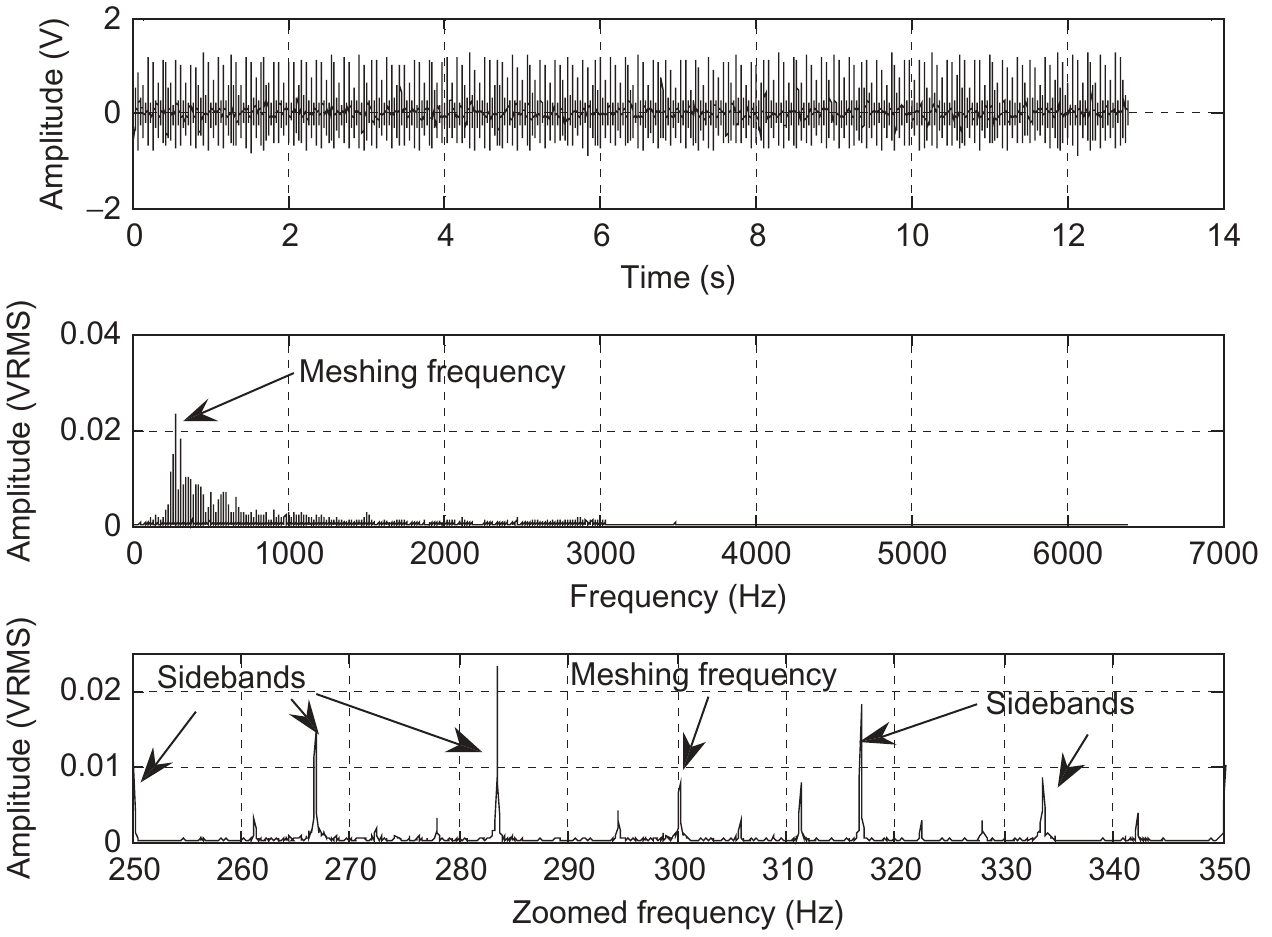
\includegraphics[width=0.8\linewidth]{img/img13}
	\end{figure}
\end{frame}

\subsection{Digital image enhancement}

\begin{frame}{Image enhancement}
	\begin{figure}
		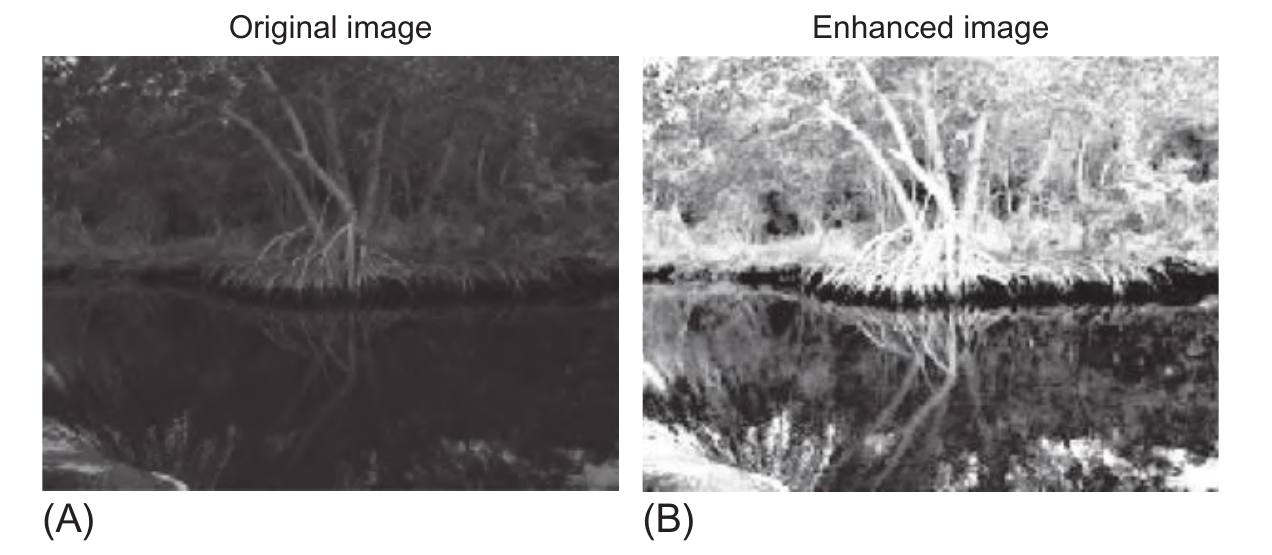
\includegraphics[width=\linewidth]{img/img14}
	\end{figure}
\end{frame}

\subsection{Applications of digital signal processing}

\begin{frame}{Applications of digital signal\\processing}
	\begin{figure}
		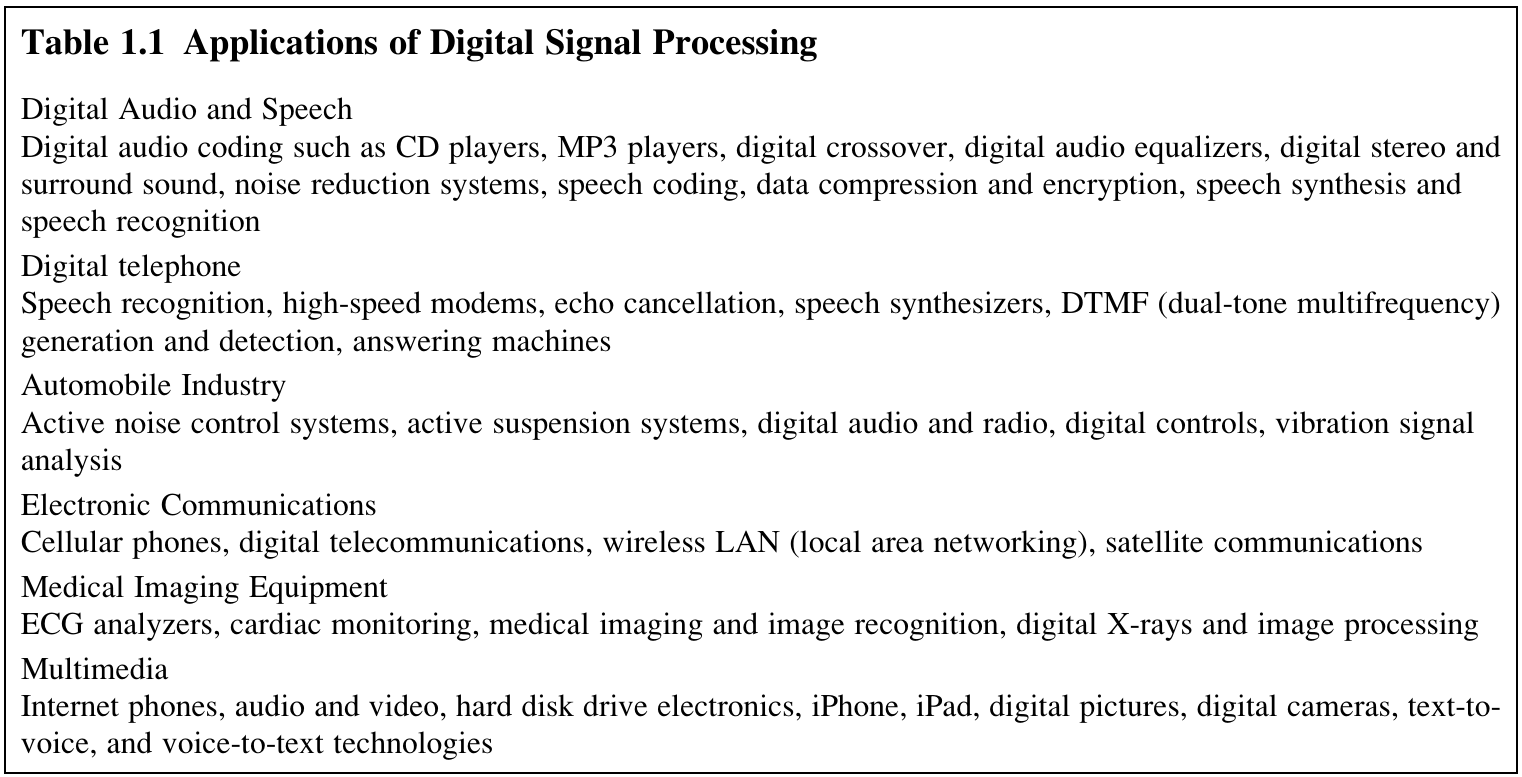
\includegraphics[width=\linewidth]{img/img15}
	\end{figure}
\end{frame}

\end{document}
